\section{Preliminaries}
\frame{\tableofcontents[currentsection]}

\begin{frame}
  \frametitle{Preliminaries}
  \begin{itemize}
    \item This section is mostly a recap
    \item We include it anyway as a reminder
    \item It also establishes context
  \end{itemize}
\end{frame}

\subsection{Terminology}
\frame{\tableofcontents[currentsubsection]}

\begin{frame}
  \frametitle{Terminology: Least/Most Significant Bit}
  \begin{itemize}
    \item Rightmost bit is called \emph{least significant bit} (MSB)
    \item Leftmost bit is called \emph{most significant bit} (LSB)
  \end{itemize}
  \begin{overprint}
    \onslide<1|handout:1>
    \structure{\texttt{uint8\_t}}
    \begin{center}
      \begin{tikzpicture}
        \draw (0,0) grid (8,1);
        \foreach[evaluate={\i-0.5} as \x] \i in {1,...,8} {
          \tikzmath{
            int \v;
            \v = random(0, 1);
          }
          \node at (\x, 0.5) {\v};
        }

        \node[anchor=north] (msb) at (0.5,-0.5) {most significant bit};
        \draw[-latex] (msb) -- (0.5,0);

        \node[anchor=north] (lsb) at (7.5,-0.5) {least significant bit};
        \draw[-latex] (lsb) -- (7.5,0);
      \end{tikzpicture}
    \end{center}

    \onslide<2|handout:0>
    \structure{\texttt{uint16\_t}}
    \begin{center}
      \begin{tikzpicture}
        \draw (0,0) grid[step=0.5cm] (8,0.5);
        \foreach[evaluate={\i/2-0.25} as \x] \i in {1,...,16} {
          \tikzmath{
            int \v;
            \v = random(0, 1);
          }
          \node[font=\tiny] at (\x, 0.25) {\v};
        }

        \node[anchor=north] (msb) at (0.25,-0.5) {most significant bit};
        \draw[-latex] (msb) -- (0.25,0);

        \node[anchor=north] (lsb) at (7.75,-0.5) {least significant bit};
        \draw[-latex] (lsb) -- (7.75,0);
      \end{tikzpicture}
    \end{center}

    \onslide<3|handout:0>
    \structure{\texttt{uint32\_t}}
    \begin{center}
      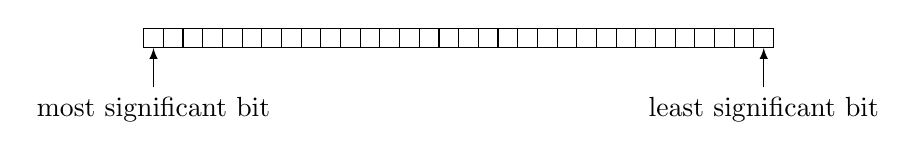
\begin{tikzpicture}
        \draw (0,0) grid[step=0.25cm] (8,0.25);
        \node[anchor=north] (msb) at (0.125,-0.5) {most significant bit};
        \draw[-latex] (msb) -- (0.125,0);

        \node[anchor=north] (lsb) at (7.875,-0.5) {least significant bit};
        \draw[-latex] (lsb) -- (7.875,0);
      \end{tikzpicture}
    \end{center}
  \end{overprint}
\end{frame}

\begin{frame}
  \frametitle{Terminology: Nibble}
  \begin{itemize}
    \item A \emph{byte} contains 8 bits
    \item A \emph{nibble} contains 4 bits
    \item One byte consists of two nibbles
  \end{itemize}
  \vskip4mm
  \begin{center}
    \begin{tikzpicture}[scale=0.75,transform shape]
      \begin{scope}
        \node[anchor=east] at (-0.5,0.5) {nibble};
        \draw (0,0) grid (4,1);
        \foreach[evaluate={\i-0.5} as \x] \i in {1,...,4} {
          \tikzmath{
            int \v;
            \v = random(0, 1);
          }
          \node at (\x, 0.5) {\v};
        }
      \end{scope}
      \begin{scope}[yshift=-1.5cm]
      \node[anchor=east] at (-0.5,0.5) {byte};
        \draw (0,0) grid (8,1);
        \foreach[evaluate={\i-0.5} as \x] \i in {1,...,8} {
          \tikzmath{
            int \v;
            \v = random(0, 1);
          }
          \node at (\x, 0.5) {\v};
        }
      \end{scope}
    \end{tikzpicture}
  \end{center}
\end{frame}


\subsection{Integers}
\frame{\tableofcontents[currentsubsection]}

\begin{frame}
  \frametitle{Integers}
  \begin{itemize}
    \item \cpp\ offers both signed and unsigned integers
    \item For clarity's sake, examples will use 8-bit integers
    \item But same is applicable on 16, 32, 64, \dots bit integers
  \end{itemize}
\end{frame}

\begin{frame}
  \frametitle{Signed Integers}
  \begin{itemize}
    \item MSB is used to represent sign
    \item If MSB = \texttt{0}, then number is positive ($\geq 0$)
    \item If MSB = \texttt{1}, then number is negative ($< 0$)
    \item Java only offers signed integers
  \end{itemize}
  \begin{center}
    \begin{tikzpicture}[scale=0.75,transform shape]
      \draw (0,0) grid (8,1);
      \foreach[evaluate={\i-0.5} as \x] \i in {1,...,8} {
        \tikzmath{
          int \v;
          \v = random(0, 1);
        }
        \node at (\x, 0.5) {\v};
      }
      \draw[|-|] (0,-0.25) -- (1,-0.25) node[midway,below,font=\tiny] {sign bit};
      \draw[|-|] (1,-0.25) -- (8,-0.25) node[midway,below,font=\tiny] {value};
    \end{tikzpicture}
  \end{center}
  \begin{center}
    \begin{tabular}{cccc}
      \toprule
      \textbf{Type} & \textbf{\# Bits} & \textbf{Lowest} & \textbf{Highest} \\
      \midrule
      \texttt{int8\_t} & 8 & $-128$ & $127$ \\
      \texttt{int16\_t} & 16 & \num{-32768} & \num{32767} \\
      \texttt{int32\_t} & 32 & $-2^{31}$ & $2^{31}-1$ \\
      \texttt{int64\_t} & 64 & $-2^{63}$ & $2^{63}-1$ \\
      & $N$ & $-2^{N-1}$ & $2^{N-1}-1$ \\
      \bottomrule
    \end{tabular}
  \end{center}
\end{frame}

\begin{frame}
  \frametitle{Unsigned Integers}
  \begin{itemize}
    \item All bits are used to represent value
  \end{itemize}
  \begin{center}
    \begin{tikzpicture}[scale=0.75,transform shape]
      \draw (0,0) grid (8,1);
      \foreach[evaluate={\i-0.5} as \x] \i in {1,...,8} {
        \tikzmath{
          int \v;
          \v = random(0, 1);
        }
        \node at (\x, 0.5) {\v};
      }
      \draw[|-|] (0,-0.25) -- (8,-0.25) node[midway,below,font=\tiny] {value};
    \end{tikzpicture}
  \end{center}
  \begin{center}
    \begin{tabular}{cccc}
      \toprule
      \textbf{Type} & \textbf{\# Bits} & \textbf{Lowest} & \textbf{Highest} \\
      \midrule
      \texttt{uint8\_t} & 8 & $0$ & $255$ \\
      \texttt{uint16\_t} & 16 & \num{0} & \num{65535} \\
      \texttt{uint32\_t} & 32 & $0$ & $2^{32}-1$ \\
      \texttt{uint64\_t} & 64 & $0$ & $2^{64}-1$ \\
      & $N$ & $0$ & $2^{N}-1$ \\
      \bottomrule
    \end{tabular}
  \end{center}
\end{frame}


\subsection{Number Notations}
\frame{\tableofcontents[currentsubsection]}

\begin{frame}
  \frametitle{Integer Literals}
  \begin{itemize}
    \item Literal: code representation of a value
    \item Programming languages offer literals for built-in types
  \end{itemize}
  \vskip4mm
  \structure{Examples}
  \begin{center}
    \begin{tabular}{ll}
      \toprule
      \textbf{Type} & \textbf{Example} \\
      \midrule
      String & \texttt{"abc"} \\
      Boolean & \texttt{true} \\
      Integer (decimal) & \texttt{51} \\
      Integer (hexadecimal) & \texttt{0xA12F} \\
      Integer (binary) & \texttt{0b10010101} \\
      \bottomrule
    \end{tabular}
  \end{center}
\end{frame}

\begin{frame}
  \frametitle{Hexadecimal}
  \begin{itemize}
    \item A nibble contains 4 bits
    \item It can represent 16 different values
    \item This corresponds exactly to one hexadecimal digit
  \end{itemize}
  \begin{columns}[t]
    \begin{column}{4cm}
      \begin{center}
        \begin{tabular}{cc}
          \toprule
          \textbf{Nibble} & \textbf{Hex digit} \\
          \midrule
          \texttt{0b0000} & \texttt{0x0} \\
          \texttt{0b0001} & \texttt{0x1} \\
          \texttt{0b0010} & \texttt{0x2} \\
          \texttt{0b0011} & \texttt{0x3} \\
          \texttt{0b0100} & \texttt{0x4} \\
          \texttt{0b0101} & \texttt{0x5} \\
          \texttt{0b0110} & \texttt{0x6} \\
          \texttt{0b0111} & \texttt{0x7} \\
          \bottomrule
        \end{tabular}
      \end{center}
    \end{column}
    \begin{column}{4cm}
      \begin{center}
        \begin{tabular}{cc}
          \toprule
          \textbf{Nibble} & \textbf{Hex digit} \\
          \midrule
          \texttt{0b1000} & \texttt{0x8} \\
          \texttt{0b1001} & \texttt{0x9} \\
          \texttt{0b1010} & \texttt{0xA} \\
          \texttt{0b1011} & \texttt{0xB} \\
          \texttt{0b1100} & \texttt{0xC} \\
          \texttt{0b1101} & \texttt{0xD} \\
          \texttt{0b1110} & \texttt{0xE} \\
          \texttt{0b1111} & \texttt{0xF} \\
          \bottomrule
        \end{tabular}
      \end{center}
    \end{column}
  \end{columns}
\end{frame}

\begin{frame}
  \frametitle{Hexadecimal}
  \begin{center}
    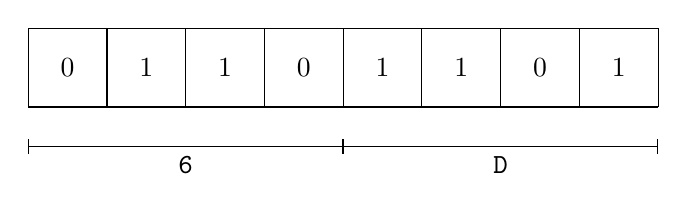
\begin{tikzpicture}
      \draw (0,0) grid (8,1);
      \foreach[count=\i,evaluate={\i-0.5} as \x] \v in {0,1,1,0,1,1,0,1} {
        \node at (\x, 0.5) {\v};
      }

      \draw[|-|] (0,-0.5) -- ++(4,0) node[midway,below] {\texttt{6}};
      \draw[|-|] (4,-0.5) -- ++(4,0) node[midway,below] {\texttt{D}};
    \end{tikzpicture}
  \end{center}
  \begin{itemize}
    \item Byte consists of 2 nibbles
    \item Single byte written down as two hexadecimal digits
  \end{itemize}
\end{frame}

\begin{frame}
  \frametitle{Binary and Hexadecimal}
  \begin{itemize}
    \item Binary and hexadecimal are a good match
    \item One hex digit always corresponds to four binary digits
    \item Makes conversion between notations easy
          \begin{itemize}
            \item Bundle binary digits in groups of 4
            \item Each group can be translated to hex independently
          \end{itemize}
    \item No such nice correspondence with decimal notation
  \end{itemize}
\end{frame}

\begin{frame}
  \frametitle{Important To Remember}
  \begin{itemize}
    \item Remember the sizes
          \begin{center}
            \begin{tabular}{ccc}
              \toprule
              \textbf{Type} & \textbf{\# Hex Digits} & \textbf{Example} \\
              \midrule
              \texttt{uint8\_t} & 2 & \texttt{0x25} \\
              \texttt{uint16\_t} & 4 & \texttt{0xA452} \\
              \texttt{uint32\_t} & 8 & \texttt{0x80F135E5} \\
              \bottomrule
            \end{tabular}
          \end{center}
          \vskip2mm
    \item Remember these special values
          \begin{itemize}
            \item \texttt{0x00 == 0b00000000}
            \item \texttt{0xFF == 0b11111111}
          \end{itemize}
  \end{itemize}
\end{frame}
